\documentclass{amsart}

%\usepackage{fullpage}
\usepackage{amsmath,amssymb,amsfonts,amsthm,stmaryrd}
%\usepackage{stmaryrd}

\usepackage{mathpazo} % math & rm
\linespread{1.05}        % Palatino needs more leading (space between lines)
\usepackage[scaled]{helvet} % ss
\usepackage{courier} % tt
\normalfont
\usepackage[T1]{fontenc}

\usepackage{tikz-cd}

\usepackage{todonotes}
\usepackage{lscape}
\usepackage{rotating}

\usepackage{cleveref}

\newcommand{\Z}{\mathbb Z}
\renewcommand{\S}{\mathbb S}
\newcommand{\F}{\mathbb F}
\newcommand{\G}{\mathbb G}
\newcommand{\R}{\mathbb R}
\newcommand{\RP}{\R\mathrm P}
\newcommand{\C}{\mathbb{C}}
\newcommand{\CP}{\C\P}
\newcommand{\A}{\widehat{\mathbb{A}}}
\newcommand{\Q}{\mathbb{Q}}
\newcommand{\M}{\mathcal{M}}
\newcommand{\FH}{\textbf{FH}}
\newcommand{\CH}{\textbf{CH}}
\renewcommand{\L}{\mathcal{L}}
\renewcommand{\H}{\mathcal{H}}
\renewcommand{\P}{\mathbb{P}}
\newcommand{\W}{\mathbb W}
\newcommand{\m}{m}

\newcommand{\<}{\langle}
\renewcommand{\>}{\rangle}
\newcommand{\sm}{\wedge}
\newcommand{\Susp}{\Sigma}
\renewcommand{\phi}{\varphi}
\renewcommand{\epsilon}{\varepsilon}
\newcommand{\eps}{\varepsilon}
\newcommand{\mmod}{/\!\!/}
\newcommand{\co}{\colon\thinspace}
\newcommand{\into}{\hookrightarrow}
\newcommand{\cotensor}{\square}

\newcommand{\context}[1]{\mathcal{M}_{#1}}
\newcommand{\CatOf}[1]{\mathsf{#1}}
\newcommand{\ps}[1]{\llbracket{#1}\rrbracket}
\newcommand{\moduli}[1]{\mathcal{M}_{\mathbf{#1}}}
\newcommand{\OS}[2]{\smash{\underline{#1}}_{#2}}
\newcommand{\sheaf}[1]{\mathcal{#1}}

\newcommand{\Spin}{\mathit{Spin}}
\newcommand{\String}{\mathit{String}}
\newcommand{\TMF}{\mathit{TMF}}
\newcommand{\tmf}{\mathit{tmf}}
\newcommand{\BP}{\mathit{BP}}
\newcommand{\MU}{\mathit{MU}}
\newcommand{\Tate}{\mathrm{Tate}}
\newcommand{\gl}{\mathit{gl}}
\newcommand{\GL}{\mathit{GL}}
\newcommand{\perf}{\mathrm{perf}}
\newcommand{\gpd}{\mathrm{gpd}}

\DeclareMathOperator{\Spec}{Spec}
\DeclareMathOperator{\Spf}{Spf}
\DeclareMathOperator{\Sch}{Sch}
\DeclareMathOperator{\colim}{colim}
\DeclareMathOperator{\End}{End}
\DeclareMathOperator{\Div}{Div}
\DeclareMathOperator{\SDiv}{SDiv}
\DeclareMathOperator{\Sq}{Sq}
\DeclareMathOperator{\Sym}{Sym}
\DeclareMathOperator{\Aut}{Aut}
\DeclareMathOperator{\Def}{Def}
\DeclareMathOperator{\Pic}{Pic}

% \numberwithin{equation}{section}

\theoremstyle{plain}
\newtheorem*{theorem}{Theorem}
\newtheorem*{proposition}{Proposition}
\newtheorem*{lemma}{Lemma}
\newtheorem*{corollary}{Corollary}
\newtheorem*{conjecture}{Conjecture}
\theoremstyle{definition}
\newtheorem*{definition}{Definition}
\newtheorem*{construction}{Construction}
\newtheorem*{warning}{Important Warning}
\theoremstyle{remark}
\newtheorem*{remark}{Remark}
\newtheorem*{example}{Example}

\title{Formal Geometry in Algebraic Topology}
\author{Eric Peterson}

\begin{document}

\maketitle

\textbf{Class information}

\vspace{2\baselineskip} \noindent \textit{Meeting times: }
Spring 2016, MWF 12pm--1pm.

\vspace{2\baselineskip} \noindent \textit{Goals: }
The primary goal of this class is to teach students to view results in algebraic topology through the lens of (formal) algebraic geometry.

\vspace{2\baselineskip} \noindent \textit{Grading: }
This class won't have any official assignments. I'll give references as readings for those who would like a deeper understanding, though I'll do my best to ensure that no extra reading is required to follow the arc of the class.

I do want to assemble course notes from this class, but it's unlikely that I will have time to type \emph{all} of them up. Instead, I would like to ``crowdsource'' this somewhat: I'll type up skeletal notes for each lecture, and then we as a class will try to flesh them out as the semester progresses. As incentive to help, those who contribute to the document will have their name included in the acknowledgements, and those who contribute \emph{substantially} will have their name added as a coauthor. Everyone could use more CV items.



\newpage

\section{Jan 25}

The goal of this class is to communicate a certain \textit{weltanschauung} uncovered in pieces by many different people working in bordism theory, and the goal just for today is to tell a story about one theorem where it is especially apparent.

To begin, recall that a bordism theory $MX$, where $X$ is some suitable family of structure groups $X_n \to O(n)$, is a homology theory similar to singular homology but where the chains are constructed from $X$--structured manifolds and their boundaries.  The coefficient ring of $MX$, or its value $MX_*(*)$ on a point, gives the ring of $X$--bordism classes, and generally $MX_*(Y)$ of some space $Y$ gives a kind of ``bordism in families''.  There are evident comparison morphisms for the most ordinary kinds of bordism, given by replacing a chain of manifolds with an equivalent simplicial chain: \[MO \to H\Z/2, \quad MSO \to H\Z.\] The first one is essentially an equivalence, but the second one is quite far from being an equivalence. More intriguingly, for $X = e$ the trivial structure group, the Pontryagin--Thom construction gives an equivalence $Me \xrightarrow{\simeq} \S$, and so it is possible (and some people have indeed taken up this viewpoint) that stable homotopy theory can be done solely through the lens of ``framed bordism''.

I'm a stable homotopy theorist rather than a differential topologist, and so I prefer to view this the other way: the sphere spectrum $\S$ often appears in my life as a natural object, and I will sometimes replace it by $Me$, the framed bordism spectrum.  For example, often I encounter a ring spectrum $E$, and it comes equipped with a unit map $\S \to E$, which I can reconsider as a ring map $\S = Me \to E$.

This is the situation Ochanine and Witten found themselves in some decades ago. Ochanine had proven the following mysterious theorem:

\begin{theorem}[Ochanine]
There is a cobordism invariant $o(M)$ of an oriented manifold $M$ which is a level $2$ modular form. It is probably multiplicative: if $F \to E \to M$ is a suitable fibration, then $o(E) = o(F) \cdot o(M)$.
\end{theorem}

\noindent 




theories of integration




The structure of the class will be, more or less, to work through a sequence of case studies where this perspective on algebraic topology shines through most brightly.  We'll start by working through Thom's calculation of the homotopy of $MO$, which simultaneously holds the attractive features of being free of technical complexity while revealing essentially all of the structural complexity.  Having seen that through to the end, we'll then work on reinforcing our technical underpinnings, and then we'll venture on to other examples.






The stated goal of this class is to study something called the ``$\sigma$--orientation'', due in various incarnations to Ochanine, Witten, Ando--Hopkins--Strickland, Ando--Strickland, Ando--Hopkins--Rezk, and probably others.



\begin{theorem}[Witten]
Ochanine's genus is definitely multiplicative. Also, if $M$ is a Spin manifold such that twice the first Pontryagin class vanishes, then $o(M)$ can be refined to a level $1$ modular form $w(M)$.
\end{theorem}




\begin{theorem}[Ando--Hopkins--Strickland]
If $E$ is an ``elliptic cohomology theory'', then there is a canonical map $M\String \to E$ called the $\sigma$--orientation.  If $E$ is taken to be Tate $K$--theory $K^{\Tate}$, then the induced map $M\String_* \to K^{\Tate}_*$ is (the $q$--expansion of) Witten's genus.
\end{theorem}

A meta-goal of this class is to focus on how the homotopical $\sigma$--orientation was actually first constructed: using formal geometry.  Their original proof begins with a reduction to understanding maps \[MU[6, \infty) \to E\] and then working to show that they can complete the missing arrow in the diagram
\begin{center}
\begin{tikzcd}
MU[6, \infty) \arrow{r} \arrow{rd} & M\String \arrow[densely dotted]{d} \\
& E.
\end{tikzcd}
\end{center}
Leaving aside the extension problem for the moment, their main theorem is the following description of the cohomology ring $E^* MU[6, \infty)$:
\begin{theorem}[Ando--Hopkins--Strickland]
For $E$ an even--periodic cohomology theory, \[\Spec E_* MU[6, \infty) \cong C^3(\G_E; \sheaf I(0)),\] where ``$C^3(\G_E; \sheaf I(0))$'' is a certain scheme.  When $E$ is taken to be elliptic, this furnishes the scheme with a canonical point, and hence gives a preferred class $MU[6, \infty) \to E$.
\end{theorem}
\noindent Our real goal is to understand theorems like these. The class will be made up of case studies where we investigate some phenomenon in algebraic topology and recast its solution in terms of formal geometry. The overriding theme of the class will be that this is a good organizing principle that gives us one avenue of insight into how homotopy theory functions. 





Theories of integration

Framed bordism agrees with the sphere spectrum


\section{Material for lecture}

The cohomology of a qc sheaf pushed forward from a scheme to a stack along a cover agrees with just the cohomology over the scheme. (In the case of $* \to * \mmod G$, this probably uses the cospan $* \to * \mmod G \leftarrow *$ with pullback $G$...)

Akhil Mathew has notes from an algebraic geometry class ( https://math.berkeley.edu/{\textasciitilde}amathew/232b.pdf ) where lectures 3--5 address the theorem of the cube.

Equivalences of various sorts of cohomologies: Ext in modules and quasicoherent cohomology (goodness. Hartshorne, I suppose); Ext in comodules and quasicoherent cohomology on stacks (COCTALOS Lemma 12.4); quasicoherent cohomology on simplicial schemes (Stacks project 09VK).

\section{Jan 27}

\section{Jan 29}

\section{Feb 1}

\section{Feb 3}

\section{Feb 5}

\section{Feb 8}

\section{Feb 10}

\section{Feb 12}

\section{Feb 17}

\section{Feb 19}

\section{Feb 21}

\section{Feb 24}

\section{Feb 26}

\section{Feb 28}

\section{Mar 2}

\section{Mar 4}

\section{Mar 7}

\section{Mar 9}

\section{Mar 11}

\section{Mar 21}

\section{Mar 23}

\section{Mar 25}

\section{Mar 28}

\section{Mar 30}

\section{Apr 1}

\section{Apr 4}

\section{Apr 6}

\section{Apr 8}

\section{Apr 11}

\section{Apr 13}

\section{Apr 15}

\section{Apr 18}

\section{Apr 20}

\section{Apr 22}

\section{Apr 25}

\section{Apr 27}

\section{Apr 29}

\section{May 2}

\section{May 4}




\newpage

\section{Ideas}
\begin{enumerate}
\item Overview of the class. (Orientations and theories of integration. Statement of the $\sigma$--orientation.)

\textsc{Case study: mod--$2$ homology}
\item Sheaves and formal schemes. The Steenrod algebra and $\context{H\F_2}$.
\item The mod--$2$ Adams spectral sequence. Sheaf cohomology. 
\item The sheaf $\context{H\F_2}(MO)$ and $\pi_* MO$.

\textsc{Introduction to the chromatic program}

\item Neil's $X_E$ construction for a general $E$. Formal schemes and formal groups. Basic theorems on formal varieties.
\item Simplicial presheaves, definition of the context. Homological and cohomological versions. Thom isomorphisms, and Quillen's theorem on $\context{\MU}$.
\item Structure theorems on $\moduli{fg}$. The picture. The definition of $K$-- and $E$--theories.
\item Group schemes and Hopf algebras. Finite dimensional Hopf algebras form an abelian category. Dieudonn\'e theory.
\item The periodicity and thick subcategory theorems. Bousfield localization, chromatic localizations and their properties, chromatic convergence.
\item $E(1)$--local homotopy of the sphere.

\textsc{The $\sigma$--orientation}

\item Thom spectra, line bundles, and divisors
\item The nonrigid, complex $\sigma$--orientation
\item Cohomological versions of AHS: $BU[2k, \infty)_E$.
\item The real version of the $\sigma$--orientation: $B\String_E$
\item Singer--Stong calculation of $H^* BU[2k, \infty)$.

\textsc{Power operations}

\item Ando, Hopkins, Strickland on $H_\infty$--orientations and the norm condition
\item The rigid, real $\sigma$--orientation: AHR. Its effect in homology.
\item The Rezk logarithm and the Bousfield--Kuhn functor
\item Statement of Lurie's characterization of $\TMF$, using this to determine a map from $M\String$ by AHR
\item Dylan's paper on String orientations
\item Matt's calculation of $E_\infty$--orientations of $K(1)$--local spectra using the short free resolution of $MU$ in the $K(1)$--local category

---------------------
\item Cartier duality
\item Subschemes and divisors
\item Coalgebraic formal schemes
\item \textit{Forms of $K$--theory}, Elliptic spectra, Tate $K$--theory, $\TMF$
\item The Ravenel--Wilson calculation, Weil pairings, Neil's MO answer about $H_* K(\Z, 3)$
\item $\sigma$ restricted to $K_{\Tate}$
\item What are $\Theta$--structures for geometers studying abelian varieties?
\item What are Weil pairings for geometers?
\item The Atiyah--Bott--Shapiro orientation (Is there a complex version of this? I understand it as a splitting of $M\Spin$...)
\item The HLP conjecture
\item Sinkinson's calculation and $M\BP\<m\>$--orientations
\item Hovey--Ravenel on nonorientations of $E_n$ by $MO[k, \infty)$. Other things in H--R?
\item Wood's cofiber sequence and $KO_{(p \ge 3)}$
\item The Serre--Tate theorem
\item The thick subcategory theorem.  Nilpotence and periodicity.
\item The chromatic spectral sequence, computations of $\pi_* L_{E(n)} \S$ for low $n$.
\item The fundamental domain of $\pi_{GH}$
\item Orientations and the functor $\gl_1$.
\end{enumerate}

\section{------------------------}



\section{Resources}

Ando, Hopkins, Strickland (Theorem of the Cube)

Ando, Hopkins, Strickland ($H_\infty$ map)

Ando, Strickland

Ando, Hopkins, Rezk

Barry Walker's thesis

Bill Singer's thesis, Bob Stong's \textit{Determination}

Hughes, Lau, Peterson

Morava's \textit{Forms of $K$--theory}

Neil's Functorial Philosophy for Formal Phenomena

Ravenel, Wilson

Kitchloo, Laures, Wilson


\section{$\context{H\F_2}(MO)$}

Hood made the following nice observation. $MO^{H\F_2}$ is the scheme of coordinates on $\RP^\infty_{H\F_2}$, with coordinate ring $\F_2[x_1, x_2, \ldots]$ and corresponding series $f(t) = \sum_{n=1}^\infty x_{n-1} t^n$ and $x_0 = 1$ implicit. This identification is equivalent to Adams's observation that $MO$ is the ``free homotopy ring spectrum'' on $MO(1)$ his sense. Then, $\Spec \mathcal{A}_* = \underline{\operatorname{Aut}}(\widehat{\G}_a)$ acts on this by coordinate changes (and we can pick a left-- or right--action as we see fit). If we pick an action by postcomposition, then we can do the following nice thing: set $f(t) = f_2(t) + g(t)$, where $f_2(t)$ contains just the terms in degrees perfect powers of $2$. Then $f_2^{-1}(f(t))$ is another coordinate with no terms in degrees perfect powers of $2$, and any nontrivial automorphism applied to this ``reduced'' series will re-introduce terms in degrees perfect powers of $2$.  So, this is a canonical form for the series under the $\underline{\operatorname{Aut}}(\widehat{\mathbb G}_a)$--action which admits no further automorphisms. It should follow that $H^*(\context{H\F_2}; \context{H\F_2}(MO))$ has amplitude $0$ and takes the form $\F_2[x_j \mid j \ne 2^n - 1]$, i.e., whose generating function is arbitrary other than having no terms in degrees perfect powers of $2$.

This means that the Adams spectral sequence degenerates and this computes $\pi_* MO$.  (It would be nice to interpret this in terms of a logarithm on $\RP^\infty_{H\F_2}$.)  It also means that the Hurewicz map is injective, hence that $MO$ is a retract of $H\F_2 \sm MO$, hence that $MO$ is an $H\F_2$--module, hence that $MO$ is a wedge of shifts of $H\F_2$.


\newpage
\newpage
\newpage

\vspace{20\baselineskip}

\begin{center}
What follows are notes from other talks I've given about quasi-relevant material which can probably be cannibalized for this class.
\end{center}



% -*- root: main.tex -*-

\newpage









\section*{-------------------------}




ideas for open questions which i ended up not using:


the Goerss--Hopkins--Miller theorem\footnote{Davis and Torii are responsible for the $(E_n \hat\wedge X)^{h\mathbb G_n} \simeq L_{K(n)} X$ equivalence.}

$K(n)$--local homotopy groups

the telescope conjecture

equivariant $E$--theory

connection to $TMF$ and higher orientations

character theories, transchromatic phenomena generally

Dieudonn\'e: Presentation of the endomorphism ring of the generic height $d$ law.


\newpage
\section*{-----------------------------}

Nat's MPIM notes

(The first thing Nat says is that Vesna already introduced $tmf$ in the first two talks and that Tobi was going to introduce the chromatic program in the fifth talk.)

\section*{Introduction: K--theory}
    \subsection*{Quillen's theorem}
    \subsection*{The (integral) Conner--Floyd isomorphism}
    \subsection*{Total power operations in equivariant K--theory}
    \subsection*{Hopf invariant one}

\section*{Morava E--theory and the LEFT}
    \subsection*{Examples of formal group laws}
    \subsection*{Lubin--Tate deformation theory}
    \subsection*{Definition of E--theory using LEFT}

\section*{Morava E--theory as a commutative ring spectrum}
    \subsection*{The Goerss--Hopkins--Miller theorem}
    \subsection*{Devinatz--Hopkins on fixed point spectral sequences}
    \subsection*{TMF restricted to the supersingular locus}
    \subsection*{The Goerss--Henn--Mahowald--Rezk resolution}

\section*{Morava E--theory and algebraic geometry}
    \subsection*{$\mathbb C \mathrm P^\infty_E$ as a formal scheme}
    \subsection*{$BA^*_E$ and $BU(n)_E$ as formal schemes}
    \subsection*{Strickland's theorem on finite symmetric groups}
    \subsection*{Power operations and Ando's theorem}

\section*{Morava $E$--theory and representation theory}
    \subsection*{The case for equivariant and $p$--adic $K$--theory}
    \subsection*{The classical Chern character}
    \subsection*{The HKR character map}


\newpage

\section*{Formal schemes for spaces}



\section*{$BU[2k, \infty)$}

Given these descriptions, it's easy to take the colimit in $n$ to get a description of $BU_E$: just as $BU$ classifies stable vector bundles of virtual rank zero, $BU_E \cong \Div_0 \CP^\infty_E$ classifies stable divisors of virtual weight zero.  Eliminating this weight condition, we also have $(BU \times \Z)_E \cong \Div \CP^\infty_E$.  These two spaces suggest a new avenue of generalization, as they are both spaces in the connective complex $K$--theory spectrum:
\begin{align*}
BU \times \Z & \simeq \OS{kU}{0}, & BU & \simeq \OS{kU}{2}.
\end{align*}
The next space in this sequence is also very accessible.  It lies in a fiber sequence\todo{Does is map $\OS{kU}{4} \to \OS{kU}{2}$ a map of of infinite loopspaces?}
\begin{center}
\begin{tikzcd}
BSU \arrow{r} \arrow[-,double]{d} & BU \arrow[-,double]{d} \arrow{r}{\det} & BU(1) \arrow[-,double]{d} \\
\OS{kU}{4} \arrow{r} & \OS{kU}{2} \arrow{r} & \CP^\infty.
\end{tikzcd}
\end{center}
For complex--orientable $E$, the associated Serre spectral sequence is collapsing and we have an induced short exact sequence of group schemes
\begin{center}
\begin{tikzcd}
BSU_E \arrow{r} \arrow[-,double]{d} & BU_E \arrow{r} \arrow[-,double]{d} & BU(1)_E \arrow[-,double]{d} \\
\SDiv_0 \CP^\infty_E \arrow{r} & \Div_0 \CP^\infty_E \arrow{r}{\sigma} & \CP^\infty_E,
\end{tikzcd}
\end{center}
where $\sigma$ is the summation map and ``$\SDiv$'' denotes ``special divisors'', i.e., those which sum to zero.

After this space, things get complicated quickly.  The fiber sequence \[K(\Z, 3) \to BU[6, \infty) \to BSU\] has a somewhat accessible Serre spectral sequence, but the higher analogues do not.  In his PhD thesis, Bill Singer completed this calculation for mod--$p$ cohomology using carefully iterated Eilenberg--Moore spectral sequences:

\begin{theorem}[Bill Singer; Bob Stong]
Take $E = H\F_2$.  There is an isomorphism \[H\F_2^*(BU[2k,\infty)) = \frac{H\F_2^*(BU)}{\F_2[\theta_{2i} \mid \sigma_2(i - 1) < k - 1]} \otimes \operatorname{Op}[\Sq^3 \iota_{2k-3}],\] where ``$\operatorname{Op}[\Sq^3 \iota_{2k-3}]$'' denotes the smallest sub-Steenrod-Hopf-algebra of $H\F_2^*(K(\Z, 2k-3))$ containing $\Sq^3 \iota_{2k-3}$ and $\theta_{2i} \equiv c_i$ modulo decomposables.
\end{theorem}

This presentation does not suggest any geometric description.  Instead, using as motivation the fact that ``$\Div$'' constructs a sort of free group scheme, Ando, Hopkins, and Strickland went looking for interesting free constructions laying around.  Taking powers of the natural map $(\L - 1): BU(1) \to BU \simeq \OS{kU}{2}$ gives an interesting map \[BU(1)^{\times k} \xrightarrow{f_k} \OS{kU}{2k} \simeq BU[2k, \infty).\]  Some properties of this map are evident: it is symmetric under permuting the domain, and restricting it to the basepoint of any of the factors collapses the map.  There is an interesting third property, most easily visible by postcomposing to $BU$.  There, the associated divisor (i.e., point in $BU_E$) takes the form $\<a_1, \ldots, a_n\> := \prod_i ([a_i] - [0])$.  We then compute:
\begin{align*}
\<a_1, \ldots, a_{n+1}\> & = ([0] - [a_1])([0] - [a_2])([0] - [a_3])\<a_4, \ldots, a_{n+1}\> \\
& = ([0] - [a_1])[a_2]([0] - [a_3])\<a_4, \ldots, a_{n+1}\> + \<a_1, a_3, \ldots, a_{n+1}\> \\
& = ([0] - [a_1])([a_2] - [a_2 + a_3])\<a_4, \ldots, a_{n+1}\> + \<a_1, a_3, \ldots, a_{n+1}\> \\
& = \<a_1, a_2, a_4, \ldots, a_{n+1}\> - \<a_1, a_2 + a_3, a_4, \ldots, a_{n+1}\> + \<a_1, a_3, a_4, \ldots, a_{n+1}\> \\
\Rightarrow \<a_2, \ldots, a_{n+1}\> - \<a_1 + a_2, a_3, \ldots, a_{n+1}\> & = \<a_1, a_2, a_4, \ldots, a_{n+1}\> - \<a_1, a_2 + a_3, a_4, \ldots, a_{n+1}\>,
\end{align*}
a kind of cocycle condition.  The most important step of this computation is the transition from the second to the third line: we used the fact that $\Div_0 \CP^\infty_E$ is an ideal for $\Div \CP^\infty_E$.  This informs the following lucky guess:

\begin{theorem}[Ando, Hopkins, Strickland]
For even--periodic cohomology theories $E$ and $k \le 3$,\footnote{At $k = 2$, this scheme is not obviously equivalent to the $\SDiv_0$ description above. To explain: the map $\delta$ factors through $\ker \sigma = \SDiv_0 \G$; we will define an inverse $\phi$. Set $\phi_n(\underline a)$ for a tuple $\underline a \in \G^n$ to be $\phi_n(\underline a) = \sum_{j=1}^n [\sigma(\underline a_{< j}), a_j].$ This turns out to be $\Sigma_n$--invariant, so one can write $\phi_\infty$. This map has $\phi_\infty(\underline a + \underline b) = \phi_\infty(\underline a) + \phi_\infty(\underline b) + [\sigma(\underline a), \sigma(\underline b)]$, so for $\underline a$ and $\underline b$ in $\ker(\sigma)$ it is a homomorphism. This is the desired inverse.} there is a diagram
\begin{center}
\begin{tikzcd}
BU(1)^{\times k}_E \arrow{rr} \arrow[dashed]{rd} & & BU[2k, \infty)_E \\
& C_k := \Sym_{\Div \CP^\infty_E}^k (\Div_0 \CP^\infty_E) \arrow{ru}{\simeq}.
\end{tikzcd}
\end{center}
\end{theorem}

This is a hard theorem: not only does that map have to be checked to be an isomorphism, but the mere existence of the symmetric power scheme needs to be checked.  It's also an incredible theorem: suppose that $E$ is an elliptic cohomology theory, so that $\CP^\infty_E$ comes with a chosen isomorphism to the formal group $\widehat{C}$ of some elliptic curve $C$.  \todo{Expand this?}  The ``theorem of the cube'' in algebraic geometry applied to $C$ furnishes us with a canonical point in $MU[6, \infty)_E$, i.e., a canonical multiplicative map $MU[6, \infty) \to E$.  Morally, as $\TMF$ is the ``universal elliptic cohomology theory'', one can take a homotopy inverse limit over the various choices of $C$ to get a map \[MU[6, \infty) \xrightarrow{\sigma} \TMF.\]  This map indeed exists and is the complex--geometric version of ``the $\sigma$--orientation'' or ``Witten's string genus''.  The construction of this canonical point in $MU[6, \infty)_E$ uses in an essential way the schematic description, and it's difficult to conceive of finding the homotopy theoretic instantiation of this map without employing this language.

You'll also notice that we didn't gain many new cases with this theorem: we already understood $\OS{kU}{2k}$ for $k \le 2$, and the Ando--Hopkins--Strickland theorem applies to $k \le 3$.  At $k = 4$, we can already see what's getting in the way: the odd--degree class $\Sq^7 \Sq^3 \iota_{2k-3}$ becomes nonzero for the first time when $k = 4$, and the connection to formal geometry collapses in the presence of odd--degree information.  Nonetheless, the schemes $C_k$ continue to exist, and one can investigate them in their own right.

\begin{theorem}[Hughes, Lau, P.]
For $E = H\F_2$, the Cartier--dual scheme $C^k = \mathbb{D}(C_k)$ has an explicit and efficient presentation which can be computed as far as out as one cares.  (It isn't very pretty, though.)
\end{theorem}

Formal geometry or not, the class $f_k$ still exists, and it induces a map \[\mathcal{O} C^k \xrightarrow{f_k'} (H\F_2)_* BU[2k, \infty).\]  Given our explicit presentation, we can attempt to analyze this map.  Since the source is an even--concentrated Hopf algebra, its image in the target will also consist of even classes.  However, Singer's calculation indicates that restricting to the subalgebra of even classes in the target is not sufficient to make $f_k'$ an isomorphism.  Instead, there appears to be one other item to take into account: the Steenrod algebra $\mathcal{A}_* = \mathcal{O} \underline{\operatorname{Aut}}(\G_a)$ naturally coacts on both sides.

\begin{conjecture}[Hughes, Lau, P.]
The map $f'_k$ is $\underline{\Aut}(\G_a)$--equivariant.  Restricting the target to the Steenrod--Hopf--subalgebra of even classes \emph{which have even diagonals}, this map becomes an isomorphism.
\end{conjecture}

\noindent We've verified this computationally in thousands of bidegrees.  I can't imagine it isn't true, but I don't have a proof.  This modest conjecture naturally leads to a more seriously speculative question: is there an infinite loopspace $X_{2k}$ over $\OS{kU}{2k}$ realizing this factorization?  I have no real feelings about this either way, but I do have a philosophical soapbox to stand on.  The platform of this talk is basically that algebraic geometry can be used to capture a lot of what we do---and can even lead us to proofs of important ideas in homotopy theory, as with the $\sigma$--orientation.  Faced with the fact that these two computations don't line up, we're forced to admit one of two things: either formal geometry isn't quite capturing the natural object of complex $K$--theory and the formal geometry needs to be augmented, or complex $K$--theory isn't quite capturing the natural algebraic geometry and the spectrum needs to be augmented.

I'm tempted to give the latter viewpoint a fair shake.  Geometers seem a little confused about what, morally, comes after $BU[6, \infty)$ and $B\mathrm{String} = BO[8, \infty)$.  The Thom spectra for the spaces that come after also don't really seem to fit as nicely into homotopy theory; it's known, for instance, that $MO[9, \infty)$ can't participate in a (suitably structured) orientation for the height $3$ Morava $E$--theory.  It sure would be interesting if there were some other candidate spaces $X_{2k}$ with a tighter bond to algebraic geometry and so a better shot at achieving these goals.

Here are three immediate stray thoughts about these proposed spaces:
\begin{enumerate}
\item The spaces $X_{2k}$ cannot themselves assemble into a single infinite loopspace. A result from the 1970s of Adams and Priddy shows that any spectrum with $BU[2k, \infty)$ as its zeroth space must be a shift of $kU$.  This is a neat paper; it works by ``running the Adams spectral sequence backwards''.  Borrowing cues from it could turn up interesting results about, say, what the homotopy of $X_{2k}$ must look like.
\item Old work of Steve Wilson gives a description of all sufficiently nice $H$--spaces local to a prime: they are produces of spaces appearing as $\OS{BP\<m\>}{k}$ in the $\Omega$--spectrum for truncated Brown--Peterson theory.  It would probably be instructive to understand the cohomologies of these spaces (a calculation due to Kathleen Sinkinson) and then to compare them with the ring of functions on $C^k$.
\item Incredibly, there are tools around (due to Alexander Zabrodsky) to delete odd classes from $H$--space \emph{while preserving their $H$--spaceiness}.  These kinds of techniques could be useful here, but I suspect they'll be too crude to yield the kind of interesting result we're looking for.
\end{enumerate}







\newpage



With closed subschemes in hand, it is natural to wonder about open subschemes.  These have a more complicated definition, because the complement of a closed subscheme may not be an affine scheme.  For instance, $\A^2 \setminus \{(0, 0)\}$ is not an affine scheme --- but it is covered jointly by the affine schemes $\Spec R[x, y][x^{-1}]$ and $\Spec R[x, y][y^{-1}]$.  This behavior turns out to be generic, and one winds up at the following definition:

\begin{definition}
A subscheme $Y \to X$ of $X$ is called an open subscheme when for any pullback along a map $\Spec T \to F$ there is a collection of elements $s_k \in T$ such that for any prime $p$ in $T$ with a lift to the pullback there exists a further lift:
\begin{center}
\begin{tikzcd}
\Spec T_{(p)} \arrow[densely dotted]{d} \arrow{rd} \arrow{rdd} \\
\check{C}(\{\Spec T[s_k^{-1}]\}_k) \arrow[crossing over]{r} \arrow{rd} & \Spec T \times_F G \arrow{r} \arrow{d} & G \arrow{d} \\
& \Spec T \arrow{r} & F.
\end{tikzcd}
\end{center}
Here $\check{C}(\{\Spec T[s_k^{-1}]\}_k)$ denotes the simplicial object \[\check{C}(\{\Spec T[s_k^{-1}]\}_k) := \left\{
\begin{tikzcd}
\coprod_{k_1} \Spec T[s_{k_1}^{-1}] \arrow{r} \arrow[leftarrow,shift left=\baselineskip]{r} \arrow[leftarrow,shift right=\baselineskip]{r} & \coprod_{k_1, k_2} \Spec T\left[ \begin{array}{c} s_{k_1}^{-1} \\ , \\ s_{k_2}^{-1} \end{array} \right] \arrow[leftarrow, shift left=(2*\baselineskip)]{r} \arrow[shift left=\baselineskip]{r} \arrow[leftarrow]{r} \arrow[shift right=\baselineskip]{r} \arrow[leftarrow, shift right=(2*\baselineskip)]{r} & \cdots
\end{tikzcd}
\right\},\]
where the reader can take ``$\coprod$'' to be a formal symbol expressing the many commutative diagrams to check.
\end{definition}



\begin{remark}[{\cite[Theorem I]{Lazard}}]
In the $1$--dimensional setting, the extra symmetry condition is inoffensive: every $1$--dimensional formal group law is automatically symmetric if and only if the ground ring contains no elements which are simultaneously nilpotent and torsion.
\end{remark}



\begin{remark}\label{LieGpIntuition}
A formal group law thus arises from selecting a coordinate on a formal group and transporting the multiplication across the isomorphism.  In the motivating situation of a Lie group, we might draw the following nonsensical diagram:
\begin{center}
\begin{tikzcd}
G \times G \arrow{d} & G^\wedge_0 \times G^\wedge_0 \arrow{d} \arrow{l} & \A^n \times \A^n \arrow{d} \arrow{l}{\cong} \\
G & G^\wedge_0 \arrow{l} & \A^n, \arrow{l}{\cong}
\end{tikzcd}
\end{center}
where $G^\wedge_0$ denotes an ``infinitesimal neighborhood of $0$'' without an explicit choice of chart.  While it is not actually possible to draw such a diagram in the usual category of manifolds, formal groups give a means by which this can be studied.  The operation ``$(G, 0) \mapsto G^\wedge_0$'' is meaningful in formal schemes: for a Noetherian affine group scheme $G = \Spec A$ with zero--locus detected by the closed subscheme $\Spec (A/I) \to G$, we can associate the formal scheme \[\left\{ \Spec(A/I) \to \Spec(A/I^2) \to \cdots \to \Spec(A/I^n) \to \cdots \right\} =: G^\wedge_0 \to G.\]  The middle vertical arrow in the above diagram corresponds to the restriction of the multiplication map to this formal geometric object, and the choice of horizontal arrows (i.e., a chart) presents the multiplication as a power series (i.e., a Taylor expansion).
\end{remark}



\begin{remark}\label{WhyDeformationTheory}
The procedure of completing a scheme $X$ at a closed subscheme $Y$ is generally very useful.  It sometimes goes by the name of building the ``infinitesimal deformation space'' of the subscheme, as it has the property that if $Y \to Y' \to X$ is any nilpotent thickening of $Y$ equipped with a map to $X$ prolonging the inclusion of $Y$, then there is a factorization
\begin{center}
\begin{tikzcd}
Y \arrow{r} \arrow{d} & X^\wedge_Y \arrow{d} \\
Y' \arrow{r} \arrow[densely dotted]{ru}{\exists!} & X.
\end{tikzcd}
\end{center}
This construction is of special interest when $X$ presents a moduli problem and $Y$ selects a certain solution.  As $X^\wedge_Y$ captures the local geometry of $X$ infinitesimally closed to $Y$, it follows that $X^\wedge_Y$ describes solutions of the moduli problem which are infinitesimally close to the given solution $Y$.  This is often considerably easier to fully analyze than $X$ itself and still gives important partial information about the broader behavior of $X$.
\end{remark}

\begin{example}
The completion of the inclusion of the closed point $\Spec \F_p \to \Spec \Z$ gives the $p$--adic integers \[\Spec \F_p \to \Spf \Z_p \to \Spec \Z.\] The assertion of \Cref{WhyDeformationTheory} in this context reads that if $A$ is any complete local ring with residue field $\F_p$, then $A$ is automatically a $\Z_p$--algebra.  More generally, if $k$ is a perfect field of positive characteristic, there is an analogous object $\W(k)$, called the $p$--typical Witt vectors over $k$, so that if $A$ is a complete local ring with residue field $k$, then $A$ is automatically a $\W(k)$--algebra.  For example, for $\zeta_{p^d-1}$ a primitive $(p^d-1)$\th root of unity:
\begin{align*}
\W(\F_{p^d}) & \cong \Z_p(\zeta_{p^d-1}), & \W(\F_p) & \cong \Z_p.
\end{align*}
\end{example}



\begin{remark}\label{ExceptionalAdditiveGps}
It is common to say that the additive formal group $\G_a$ defined over a ring $R$ as above has height $\infty$, which is an obvious extension of each of the definitions of height given above.  It is also common to say that a formal group defined over a rational ring has height $0$, which --- though rational rings are not complete and local against a maximal ideal $\m$ containing $p$ --- is an extension of the geometric definition.  After all, the rational additive group has no nontrivial $p$--torsion points, so $\G_a[p]$ is of rank $1 = p^0$.
\end{remark}



\begin{remark}[{\cite[Section 24]{StricklandFPFP}}]
Since it is perhaps not immediately apparent, we indicate how $\S_d$ acts on $LT_{F_d}$.  Given a $\gamma \in \S_d$, we can construct the diagram
\begin{center}
\begin{tikzcd}
& \widetilde{F_d} \arrow[near end, densely dotted]{rr}{\widetilde{\gamma}} \arrow{dd} & & \widetilde{F_d} \arrow{dd} \\
F_d \arrow[crossing over, near end]{rr}{\gamma} \arrow{ru} \arrow{dd} & & F_d \arrow{ru} \\
& LT_{F_d} \arrow[densely dotted,near end]{rr}{\exists \gamma_{LT}} & & LT_{F_d} \\
\Spec k \arrow[-,double]{rr}{1_{LT_{F_d}}} \arrow{ru} & & \Spec k \arrow{ru} \arrow[crossing over, leftarrow]{uu} .
\end{tikzcd}
\end{center}
The dotted arrows exist because the left-most $\widetilde{F_d}$ is a versal deformation of $F_d$ and the right-most $\widetilde{F_d}$ is \emph{some} deformation of $F_d$, hence there is a map $\gamma_{LT}$ selecting it.  This gives the desired map $\S_d \to \Aut LT_{F_d}$.
\end{remark}

\begin{remark}
Let $K$ be a local number field with residue field $k$ and let $D$ be the division $K$--algebra with Hasse invariant $1/d$.  Arithmetic geometers may then recognize $\End F_d$ as a maximal order in $D$.  Algebraic topologists who were wondering where our choice of ``$d$'' to denote height came from (rather than their usual ``$n$'') now know.
\end{remark}



\begin{remark}\label{InoueRemark}
A similar statement can be made for $H\F_p$, $p \ge 3$, but care (in the guise of formal supergeometry) is required to encode the odd--degree, noncommutative Bockstein $\tau_*$ generators.  See work of Inoue for details~\cite{Inoue}.
\end{remark}



\begin{remark}
We take the opportunity to relate \Cref{QuillensTheorem} to the ordinary integral and rational homologies of $MU$.  The map $MU \to H\Z$ given by \[MU \to \colim_n MU / (c_1, c_2, \ldots, c_n)\] selects the integral additive formal group on homotopy.  The induced map $MU \sm MU \to H\Z \sm MU$ presents \[H\Z_* MU = \colim_n MU[b_1, b_2, \ldots] / (c_1, c_2, \ldots, c_n) = \Z[b_1, b_2, \ldots]\] as the universal ring with an integrally--defined strict exponential map $\exp_b(x) = \sum_j b_j x^{j+1}$ selecting another integral formal group law \[x +_b y = \exp_b( \exp^{-1}_b x + \exp^{-1}_b y).\]  By \Cref{TorsionFreeLifts}, every formal group law admits a lift to a torsion--free ring.  Furthermore, by \Cref{RationalFGLsHaveLogs} every formal group law over a rational ring has a logarithm.  It thus follows that the maps \[\pi_* MU \to H\Z_* MU \to H\Q_* MU\] are both injections.
%\todo{It might be fun to include enough information to compute the value of the Todd genus on the first few integral algebra generators of $MU_*$.}
\end{remark}



\begin{remark}
It is worth emphasizing that Landweber's theorem has two serious limitations: it only gives a homology theory rather than a spectrum, and it only applies to flat \emph{affine} maps.  In particular, this makes it very hard to arrange to use Landweber's theorem to approach nonaffine flat maps, e.g., $\moduli{ell} \to \moduli{fg}$.  Much of the work surrounding the construction of topological modular forms (alias \textit{TMF}) grapples with this issue.
\end{remark}



\begin{example}[Exceptional Morava $K$--theories]
In accordance with \Cref{ExceptionalAdditiveGps}, we define the Morava $K$--theory associated to an additive group over a field to be the Eilenberg--Mac Lane spectrum for that field.
\end{example}

\begin{remark}\label{MinimalSummands}
\Cref{LandweberExactness} bestows all these cohomology theories with $2$--periodic gradings, and this is often not minimal.  Indeed, recall from \Cref{WarningAboutGradings} that the ``$P$'' in our notation is meant to denote ``Periodic''.
\begin{enumerate}
\item $MUP$ was formed by setting $MUP = MU[u^\pm]$ with $|u| = 2$, and indeed this gives a minimal multiplicative decomposition of $MUP$ into wedge summands.
\item $BPP$ similarly decomposes multiplicatively as $BPP = BP[u^\pm]$ for some connective ring spectrum $BP$ and $|u| = 2$.  Moreover, $L_p MU$ decomposes as an infinite wedge sum of shifts of $BP$.
\item $EP(d)$ splits into a wedge of $(p^d-1)$ summands of identical $2(p^d-1)$--periodic spectra called $E(d)$.
\item $K_{F_d}$, for $F_d$ the formal group law described in \Cref{GeometricPointsOfMfg}, splits into a wedge of $(p^d-1)$ summands of identical $2(p^d-1)$--periodic spectra called $K(d)$.
\end{enumerate}
\end{remark}



\begin{remark}\label{DeeperBaseRemark}
It is tempting to think of the pro-spectrum $\{F(X_\alpha, \S)\}$ associated to a space $X$ as the primal object being studied, and that \[X_E = \{\Spec E^* X_\alpha\} = \{\Spec \pi_* (F(X_\alpha, \S) \sm_{\S} E)\}\] arises from some kind of base--change construction.  This is sometimes useful for intuition, and Mike Mandell has proven results along these lines for ordinary cohomology~\cite{MandellHZCochains,MandellHFpCochains} extending the rational results of Quillen~\cite{QuillenRational}.  However, the author does not know how to make this thought satisfyingly precise for the periodic cohomology theories $E_\Gamma$ relevant to chromatic homotopy theory.
\end{remark}




\begin{remark}
The reader may like to enrich \Cref{AnalysisOfFieldSpectra} to a statement about categories rather than a bijection of sets of isomorphism classes, but we warn that this turns out to be quite tricky.  A smattering of results in this direction can be found in work of Goerss, Hopkins, and Miller~\cite[Corollary 7.6]{GoerssHopkins}, of Ando~\cite[Theorems 1 and 5]{Ando}, and of Strickland~\cite{StricklandEthyOfBSigma}.
\end{remark}

\begin{remark}
The reader may also recall the primacy of formal groups in Lubin and Tate's explicit local class field theory.  In that context, for a local number field $K$ with ring of integers $\sheaf O_K$ and residue field $k$, the points of the maximal totally ramified abelian extension $K^{\text{trab}}$ and the Artin reciprocity morphism can both be described in terms of a certain formal group $\Gamma_K$, defined over $\sheaf O_K$ and with height prescribed by properties of $k$.  That is, some significant chunk of the arithmetic of $K$ is controlled by a background formal group.  We would like to make the vague assertion that something similar is happening here: the behavior of the field spectrum $K_\Gamma$ is again controlled by a background formal group $\Gamma \simeq \CP^\infty_{K_\Gamma}$.
\end{remark}




\section*{The $\Gamma$--local stable category}\label{KLocalCategory}

To fully employ the arithmetic geometry attached to Morava's cohomology theories, it is common to move to the associated ``local'' category --- i.e., to declare that spectra which are $K_\Gamma$--acyclic are in fact contractible, or equivalently to declare that maps which are $K_\Gamma$--homology isomorphisms are in fact weak homotopy equivalences.  This eliminates the ``pathology'' of topological phenomena which are invisible to $K_\Gamma$, and so more tightly binds the behavior of $\CatOf{Spectra}$ to $K_\Gamma$.  For reasons to be discussed in this section, we will refer to this simply as the ``$\Gamma$--local category'' with localization functor $L_\Gamma$, suppressing the letter ``$K$''.

When $\Gamma$ has finite height $d$ this category has fascinating properties, many of which will be the subject of the remainder of this paper.

\begin{center}
\textbf{From here on, we will always consider $d$ to be finite and positive unless otherwise stated.}
\end{center}

\subsection*{Continuous $E$--theory}\label{sec:ContinuousEThy}

To begin our study of the $\Gamma$--local category, we cite some bulk results which eludicate features of the localization functor:
\begin{theorem}\label{HoveyMooreSpectrumLemma}
Let $d$ be the height of $\Gamma$.
\begin{enumerate}
\item (\cite[Theorem 7.5.6]{RavenelOrangeBook}) In keeping with the above geometrically--centric notation, let $L_{\moduli{fg}^{\le d}}$ denote the Bousfield localization functor for $E(d)$.  This functor is smashing, i.e., \[L_{\moduli{fg}^{\le d}} X \simeq \left(L_{\moduli{fg}^{\le d}} \S\right) \sm X.\]
\item (\cite[Lemma 2.3]{HoveyCSC}) There is the following weak equivalence, natural in $X$: \[L_\Gamma(X) \simeq \lim_I \left(L_{\moduli{fg}^{\le d}} \S^0 \sm M_0(v^I) \sm X\right),\] where $\{M_0(v^I)\}_I$ is an inverse system of finite spectra which have bottom cell in dimension zero, which have maps $M_0(v^I) \to M_0(v^{I'})$ for $I \ge I'$, and which have \[BP_* M_0(v^I) \cong BP_* / (p^{I_0}, v_1^{I_1}, \ldots, v_{n-1}^{I_{n-1}}).\]  (Such a system is guaranteed to exist for large enough $I$ by Hopkins--Smith~\cite[Proposition 5.14]{HopkinsSmith}.)
\item (\Cref{AnalysisOfFieldSpectra}.1) The localization functor $L_\Gamma$ is an invariant of $d$ and of the characteristic $p$ of the ground field.
\item (\cite[Theorem 2.1.d, Lemma 2.3]{RavenelLocalizationWRTPeriodic}) There is a natural pullback square
\begin{center}
\begin{tikzcd}
L_{\moduli{fg}^{\le d}} X \arrow{r} \arrow{d} & L_\Gamma X \arrow{d} \\
L_{\moduli{fg}^{\le (d-1)}} X \arrow{r} & L_{\moduli{fg}^{\le (d-1)}} L_\Gamma X.
\end{tikzcd}
\end{center}
\item (\cite[Theorem 7.5.7]{RavenelOrangeBook}) For $X$ a finite spectrum, there is a natural equivalence \[X_{(p)} \simeq \lim_d L_{\moduli{fg}^{\le d}} X. \qed \]
\end{enumerate}
\end{theorem}

Before continuing, we must address one important caveat:

\begin{definition}
The homological Bousfield class of a spectrum $E$ is the collection of all spectra $X$ which have $E_* X \ne 0$.  Similarly, one can define a cohomological Bousfield class for $E$ to be the collection of all spectra $X$ which have $E^* X \ne 0$.
\end{definition}

\begin{lemma}[{\Cref{GoodCohomBousfieldClass}, \Cref{EthyFromKthy}}]\label{BadBousfieldClasses}
The cohomological Bousfield classes of $K_\Gamma$ and $E_\Gamma$ agree.  The homological Bousfield class of $E_\Gamma$ is strictly larger than the homological Bousfield class of $K_\Gamma$. \qed
\end{lemma}

\noindent This lemma has some important philosophy behind it.  \Cref{DefnEThy} and \Cref{DefnKThy} define $E$--theory as associated to the infinitesimal deformation space of $K$--theory, which suggests the presence of a cohomological Bockstein spectral sequence \[K_\Gamma(X) \otimes A \Rightarrow E_\Gamma(X).\]  Here $A$ consists of Bocksteins arising from square--zero deformation fiber sequences of the flavor
\begin{center}
\begin{tikzcd}[column sep=4.71em]
\cdots \arrow{r} & E_\Gamma / \m^{j+1} \arrow{r} \arrow{d} & E_\Gamma / \m^j \arrow{r} \arrow{d} & \cdots \\
& E_\Gamma \otimes \m^{j+1} / \m^{j+2} \arrow[-,double]{d} & E_\Gamma \otimes \m^j / \m^{j+1} \arrow{lu}{\partial,[+1]} \arrow{l}{[+1]} \arrow[-,double]{d} \\
& \underset{{\text{$x_i$ basis of $\m^{j+1} / \m^{j+2}$}}}{\bigvee} \Susp^{|x_i|} K_\Gamma & \underset{\text{$y_j$ basis of $\m^j / \m^{j+1}$}}{\bigvee} \Susp^{|y_j|} K_\Gamma \arrow{l}{\text{Bocksteins,[+1]}},
\end{tikzcd}
\end{center}
where $\m$ is the maximal ideal of the Lubin--Tate ring.  Such a spectral sequence indeed turns out to exist for the cohomology theories $K_\Gamma$ and $E_\Gamma$.  In particular, there is the following theorem:
\begin{theorem}[{\cite[Proposition 2.5]{HoveyStrickland}}]\label{GoodCohomBousfieldClass}
If $X$ is a spectrum so that $K_\Gamma^* X$ is even--concentrated, then $E_\Gamma^* X$ is pro-free and even--concentrated, so that $K_\Gamma^* X = E_\Gamma^* X \otimes_{E_\Gamma^*} E_\Gamma^* / \m$.
\end{theorem}
\begin{proof}[Proof sketch]
The differentials in the Bockstein spectral sequence take even--degree elements to odd--degree elements. By assumption there are no odd--degree elements, and hence the spectral sequence collapses at $E_1$.
\end{proof}

However, such a spectral sequence for homology (with reasonable convergence properties) is prohibited by \Cref{BadBousfieldClasses}: there are spectra with vanishing $K_\Gamma$--homology for which the $E_\Gamma$--homology is nonzero.  This is ``corrected'' by remaining inside the $\Gamma$--local category: we define the covariant functor $E_\Gamma$ by the formula \[E_\Gamma(X) := \pi_* L_\Gamma(E_\Gamma \sm X) \cong \pi_* L_\Gamma(E_\Gamma \sm L_\Gamma X).\]  The bifunctor $(X, Y) \mapsto L_\Gamma(X \sm Y)$ on $\Gamma$--local spectra determines a monoidal structure for which the localization map $L_\Gamma$ is a map of monoidal categories.  This means that the above definition of $E_\Gamma$ is the natural one for considerations internal to the $\Gamma$--local category --- and it has the pleasant extra effect of forcefully correcting the ``homological Bousfield class'' of $E_\Gamma$.  In turn, \Cref{HoveyMooreSpectrumLemma} gives the result we sought:

\begin{lemma}[{\cite[Propositions 7.10 and 8.4]{HoveyStrickland}}]\label{MilnorSeqForEThy}
There is a Milnor exact sequence \[ 0 \to \lim_j{}^1 (E_\Gamma/\m^j (\Susp^{-1} X)) \to E_\Gamma(X) \to \lim_j (E_\Gamma/\m^j(X)) \to 0,\] where the derived inverse limit is taken in abelian groups.
\end{lemma}
\begin{proof}
This is a direct corollary of \Cref{HoveyMooreSpectrumLemma} and the Milnor sequence for homotopy inverse limits (cf.\ \Cref{HomotopyMilnorSequence}).
\end{proof}

\begin{corollary}[{\cite[Proposition 8.4]{HoveyStrickland}}]\label{EthyFromKthy}
If $E_\Gamma(X)$ is pro-free then $K_\Gamma(X) \cong E_\Gamma(X) / \m_\Gamma$.  In the other direction, if $K_\Gamma(X)$ is concentrated in even dimensions, then $E_\Gamma(X)$ is pro-free.
\end{corollary}
\begin{proof}[Proof sketch]
Recall from \Cref{HoveyMooreSpectrumLemma} and \Cref{MilnorSeqForEThy} the defining sequence
\[
\pi_* L_\Gamma(E_\Gamma \sm X) \cong \pi_* \lim_I \left( M_0(v^I) \sm E_\Gamma \sm X \right).
\]
(We have used that $E_\Gamma$ is $E(d)$--local.)  The inverse system is a cofinal subsystem of the system $\pi_* \lim_I \left(E_\Gamma / (v^I) \sm X \right)$, and in the situation that $I' < 2I$ (i.e., the ideal $(v^I)$ is square--zero in $\pi_* E_\Gamma / (v^{I'})$) then the induced map $E_\Gamma / (v^{I'}) \to E_\Gamma / (v^I)$ has fiber a wedge of even--degree suspensions of $K_\Gamma$.  It follows that the long exact sequence of homotopy determining $E_\Gamma / (v^{I'})$ from $E_\Gamma / (v^I)$ degenerates into easily studied short exact sequences.
\end{proof}

\begin{remark}
The covariant functor $E_\Gamma$ does \emph{not} satisfy the axioms of a homology functor, because it does not commute with infinite colimits.  (In particular, there is a spectral sequence arising from Hovey's lemma~\cite[Lemma 2.3]{HoveyCSC} comparing the behavior of infinite colimits to a kind of derived completion~\cite{HoveyFilteredColimits}.)  Another way of viewing the difference between the two notions of $E_\Gamma$--homology is that $E_\Gamma$ is naturally expressed as an inverse limit, but the following equivalence fails, sometimes wildly: \[\pi_* \left(\left(\lim_j E_\Gamma / \m^j\right) \sm X\right) \not\cong \pi_* \lim_j \left( (E_\Gamma / \m^j) \sm X \right).\] This observation directly connects this difference to a topic in our \Cref{LimitAppendix} and in the MIT $E$--theory seminar notes~\cite[Section 14]{MITETheory}.  Nonetheless, \Cref{EthyFromKthy} is reason enough to call the covariant $E_\Gamma$ the ``correct'' notion of Morava $E$--homology, and we will unabashedly refer to it as a ``homology functor'' in the rest of this document.
\end{remark}

\begin{remark}
In the case that $K_\Gamma(X)$ is even--concentrated for a space $X$, the compact subspaces of $X$ can be used to topologize $E_\Gamma(X)$ and $E_\Gamma^*(X)$ so that they become continuously $(E_\Gamma)_*$--linearly dual to one another.  That is, the sheaf $\sheaf E_\Gamma(X)$ and the scheme $X_{E_\Gamma}$ (together with its $\Aut \Gamma$--action) contain equivalent information.
\end{remark}

Finally, we remark that $E_\Gamma$ is valued in the correct category of modules so that the functor $\sheaf E_\Gamma$ constructed by \Cref{DefnHomologyFunctorsValuedInSheaves} takes values in the correct category of sheaves:
\begin{lemma}[{\cite[Theorem 12]{StricklandGHDuality}}]\label{EthyGivesASheaf}
The functor $E_\Gamma$ is valued in modules with a continuous action of the Lubin--Tate ring (i.e., in pro-systems of modules over the finite stages of the Lubin--Tate scheme).  Additionally, these sheaves are equivariant against the action of the stabilizer group of \Cref{DefnStabilizerAlgebra}, hence they descend to the Lubin--Tate stack $\operatorname{Def}(\Gamma) \subseteq \moduli{fg}$. \qed
\end{lemma}


\subsection*{Picard--graded homotopy}\label{SectionPicardGradedHomotopy}

Picard--graded homotopy groups are a recurrent theme in homotopy theory.  For example, the $RO(G)$ grading in equivariant stable homotopy theory refers to the equivariant Picard grading, and the twists in twisted cohomology (e.g., twisted $K$--theory) refer to the Picard grading for parametrized spectra.  It also appears elsewhere in mathematics: in algebraic geometry, one studies sections of a line bundle on a projective variety rather than mere functions (i.e., sections of the trivial bundle) in order to recover further interesting data.  This, too, is an example of a Picard grading (and is where the phrase ``Picard grading'' comes from, as the the group of isomorphism classes of line bundles on a variety is called its Picard group).  The behavior of the appropriate analogue of Picard gradings in chromatic homotopy theory is very telling, and in this subsection we will recount some of what is known.

\begin{definition}\label{DefnPicardGroup}
The Picard category of a symmetric monoidal ($\infty$--)category $\CatOf{C}$ is the maximal subgroupoid of the full subcategory spanned by the $\otimes$--invertible objects.  Its connected components determine a group $\Pic \CatOf{C}$ called the Picard group of $\CatOf C$.
\end{definition}

\begin{example}[{\cite[pg. 90]{HMS} or \cite[Theorem 2.2]{StricklandInterpolate}}]\label{GlobalPicardGroup}
The Picard group of the global stable category $\CatOf{Spectra}$ is isomorphic to $\Z$ and generated by $\S^1$.
\end{example}

The Picard group of the $\Gamma$--local stable category is considerably more complicated.  Its study was initiated by Hopkins, Mahowald, and Sadofsky~\cite{HMS} at height $d = 1$, but there are now a number of results at height $d = 2$ as well; see \Cref{PicardGroupsWeKnow}.  For our present purposes, the most important of the Hopkins--Mahowald--Sadofsky results is the following theorem:

\begin{theorem}[{\cite[Theorem 1.3]{HMS}}]\label{HMSLines}
A spectrum $X$ is $\Gamma$--locally invertible if and only if $(K_\Gamma)_* X$ is $1$--dimensional as a graded vector space. \qed
\end{theorem}

\begin{remark}
Taking ``$\Pic(\CatOf{C})$'' for a moment to mean the category in \Cref{DefnPicardGroup}, this theorem can also be interpreted as asserting that the following square is a pullback in monoidal categories:
\begin{center}
\begin{tikzcd}
\CatOf{Spectra}_\Gamma \arrow{r} & \CatOf{VectorSpaces}_{K_*} \\
\Pic(\CatOf{Spectra}_\Gamma) \arrow{r} \arrow{u} & \CatOf{Lines}_{K_*} \arrow{u}.
\end{tikzcd}
\end{center}
\end{remark}

We also note that \Cref{EthyFromKthy} gives a factorization
\begin{center}
\begin{tikzcd}
\CatOf{Spectra}_\Gamma \arrow{r}{\sheaf E_\Gamma} & \CatOf{QCoh}(\Def(\Gamma)) \arrow{r}{i_0^*} & \CatOf{VectorSpaces}_{K_*} \\
\Pic(\CatOf{Spectra}_\Gamma) \arrow{u} \arrow{r} & \CatOf{LineBundles}(\Def(\Gamma)) \arrow{r}{i_0^*} \arrow{u} & \CatOf{Lines}_{K_*}. \arrow{u}
\end{tikzcd}
\end{center}
The left--hand square in this diagram is also a pullback square, but the categories in the middle column are considerably more rich than those in the right column; in particular, they contain more than one isomorphism class.  In the case of $\CatOf{LineBundles}(\Def(\Gamma))$, this corresponds to tracking the $1$--dimensional $\Aut \Gamma$--representation given by $E_\Gamma(X)$ rather than the mere $1$--dimensional vector space given by $(K_\Gamma)_*(X)$.  The following result expresses just how much more information this encodes:

\begin{lemma}[{\cite[Proposition 7.5]{HMS}}]\label{EthyDeterminesPic}
The map \[\Pic(\CatOf{Spectra}_\Gamma) \to \CatOf{LineBundles}(\Def(\Gamma))\] is injective on objects for $2p - 2 \ge d^2$ and $p \ne 2$. \qed
\end{lemma}

Throughout this document, these theorems will be our main tool which we will use to furnish $\Gamma$--locally invertible spectra.  Before proceeding to more complicated situations, we begin with a simple example in the $\G_m$--local category.  Consider the following horizontal system of cofiber sequences in the global stable category:
\begin{center}
\begin{tikzcd}
\cdots \arrow[double,-]{r} & \S^{-1} \arrow[double,-]{r} \arrow{d}{p^j} & \S^{-1} \arrow[double,-]{r} \arrow{d}{p^{j+1}} & \cdots \arrow[double,-]{r} & \S^{-1} \arrow{d} \\
\cdots \arrow{r}{p} & \S^{-1} \arrow{r}{p} \arrow{d} & \S^{-1} \arrow{r}{p} \arrow{d} & \cdots \arrow{r} & p^{-1} \S^{-1} \arrow{d} \\
\cdots \arrow[densely dotted]{r} & M^0(p^j) \arrow[densely dotted]{r} & M^0(p^{j+1}) \arrow[densely dotted]{r} & \cdots \arrow[densely dotted]{r} & M^0(p^\infty).
\end{tikzcd}
\end{center}
The row-wise homotopy colimit, pictured on the far right, is also a cofiber sequence.  The topmost object is the colimit of a sequence of identity morphisms, so is simply $\S^{-1}$.  The middle object is the colimit along iterates of the map $p$, so is, by definition, the spectrum $p^{-1} \S^{-1}$ with the $p$--self--map inverted.  Lastly, the spectrum on the bottom does not have a familiar name, so we call it $M^0(p^\infty)$.

When working $p$--locally (and so also when working $\G_m$--locally), we can see that the middle spectrum is contractible: the map $p$ on $p^{-1} \S^{-1}$ is exactly multiplication by $p$ in $K$--homology, but since the coefficient ring $K_*$ is of characteristic $p$, this is the zero map.  On the other hand, $p$ is required to be invertible, which can only mean $K_* p^{-1} \S^{-1} = 0$.  In turn, this means that the going-around map $M^0(p^\infty) \to \S^0$ is a $p$--local equivalence, and so $M^0(p^\infty)$ is an invertible spectrum, albeit not a very interesting one.\footnote{The dimension shift from $\S^{-1}$ to $\S^0$ is a homotopical reflection of the statement that the $p$-primary part of the circle group $S^1$ is the $p$--Pr\"ufer group $\Z/p^\infty = \colim_j \Z/p^j$.}

A different way of at least detecting that $M^0(p^\infty)$ is $\G_m$--locally invertible is to apply $K$--homology to the bottom row: each object in the sequence becomes a $2$--dimensional graded vector space over $K_*$, and each map from one to the next is $- \cdot p = - \cdot 0$ on the $(-1)$--graded piece and the identity on the $0$--graded piece.  Hence, the colimit is a $K_*$--line, and \Cref{HMSLines} thus assures us we have an invertible spectrum.  This is portrayed in \Cref{CellDiagramFigure}.
\begin{figure}[h]
\begin{center}
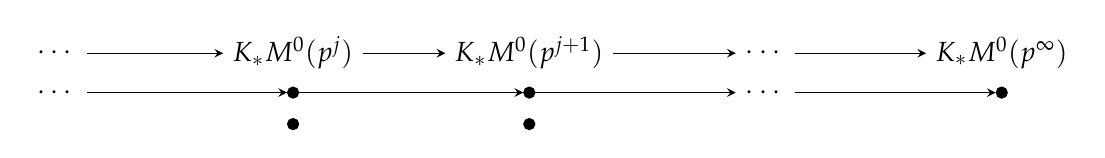
\begin{tikzpicture}[
    baseline=(current bounding box.center),
    normal line/.style={-stealth},
    node distance=3cm,
]
\node (m-1-1) {$\cdots$};
\node[right of=m-1-1] (m-1-2) {$K_* M^0(p^j)$};
\node[right of=m-1-2] (m-1-3) {$K_* M^0(p^{j+1})$};
\node[right of=m-1-3] (m-1-4) {$\cdots$};
\node[right of=m-1-4] (m-1-5) {$K_* M^0(p^\infty)$};
    \path[normal line]
        (m-1-1) edge (m-1-2)
        (m-1-2) edge (m-1-3)
        (m-1-3) edge (m-1-4)
        (m-1-4) edge (m-1-5)
;
\node[below of=m-1-1,node distance=0.5cm] (updot-1) {$\cdots$};
\node[below of=m-1-2,shape=circle,draw,node distance=0.5cm,minimum size=4pt,inner sep=0pt,fill] (updot-2) {};
\node[below of=m-1-2,shape=circle,draw,node distance=0.9cm,minimum size=4pt,inner sep=0pt,fill] (downdot-2) {};
\node[below of=m-1-3,shape=circle,draw,node distance=0.5cm,minimum size=4pt,inner sep=0pt,fill] (updot-3) {};
\node[below of=m-1-3,shape=circle,draw,node distance=0.9cm,minimum size=4pt,inner sep=0pt,fill] (downdot-3) {};
\node[below of=m-1-4,node distance=0.5cm] (updot-4) {$\cdots$};
\node[below of=m-1-5,shape=circle,draw,node distance=0.5cm,minimum size=4pt,inner sep=0pt,fill] (updot-5) {};
\path[normal line]
    (updot-1) edge (updot-2)
    (updot-2) edge (updot-3)
    (updot-3) edge (updot-4)
    (updot-4) edge (updot-5);
\end{tikzpicture}
\end{center}
\caption{``Cell diagram'' of $K_* M^0(p^\infty)$.}\label{CellDiagramFigure}
\end{figure}
This suggests a way we can modify this construction: if we insert other maps which are $K$--homology isomorphisms, then we will not harm this proof that the colimit is an invertible spectrum.  We will make use of the following results to furnish ourselves with such maps:

\begin{definition}[{\cite[Definition 1.5.3]{RavenelOrangeBook}}]
A finite spectrum $X$ is said to be of type $d$ when it is $\Gamma$--locally acyclic for all $\Gamma$ of height strictly less than $d$ and $\Gamma$--locally nontrivial for a $\Gamma$ of height exactly $d$.  (In fact, it suffices to check that acyclicity condition for any single $\Gamma$ of height $(d-1)$~\cite[Theorem 2.11]{RavenelLocalizationWRTPeriodic}.)
\end{definition}

\begin{theorem}[{Devinatz--Hopkins--Smith~\cite[Theorem 9]{HopkinsSmith}}]
A $p$--local finite spectrum $X$ is of type $d$ if and only if for $N \gg 0$ there is a map $v: \Susp^N X \to X$ which is an isomorphism in $K_\Gamma$--homology for $\Gamma$ of height $d$ and which induces the zero map in $K_\Gamma$--homology for $\Gamma$ not of height $d$.
\end{theorem}

\begin{lemma}[{Adams~\cite[Lemma 12.5]{AdamsJXIV}}]\label{AdamsSelfMaps}
The spectrum $M^0(p^{j+1})$ is type $1$ and it admits a map \[v_1^{p^j}: M^{2p^j(p-1)}(p^{j+1}) \to M^0(p^{j+1})\] which induces multiplication by $v_1^{p^j}$ in $K(1)$--homology.\footnote{Here $K(1)$ is the close cousin of $K_{\G_m}$ described in \Cref{MinimalSummands}.} Moreover, the following square commutes:
\begin{center}
\begin{tikzcd}
M^{2p^j(p-1)}(p^j) \arrow{r}{\left(v_1^{p^{j-1}}\right)^p} \arrow{d} & M^0(p^j) \arrow{d} \\
M^{2p^j(p-1)}(p^{j+1}) \arrow{r}{v_1^{p^j}} & M^0(p^{j+1}).
\end{tikzcd}
\end{center}
\end{lemma}

Selecting a $p$-adic integer $a_\infty = \sum_{j=0}^\infty c_j p^j$ with $0 \le c_j < p$, one can now construct the system \[\cdots \to M^{-|v_1| a_{j-1}}(p^j) \to M^{-|v_1| a_{j-1}}(p^{j+1}) \xrightarrow{v_1^{p^j c_j}} M^{-|v_1| a_j}(p^{j+1}) \to M^{-|v_1| a_j}(p^{j+2}) \to \cdots.\] We define $\S^{-|v_1|a_\infty}$ to be its colimit.  \Cref{HMSLines} is then sufficient to check that $\S^{-|v_1| a_\infty}$ is $\G_m$--locally invertible, but more is true:
\begin{lemma}[{\cite[Proposition 2.1]{HMS}}]\label{padicPicElements}
The above construction defines an injective continuous homomorphism of groups \[\Z_p \to \Pic(\CatOf{Spectra}_{\G_m}).\]  When $p \ge 3$ (i.e., $p \ne 2$), the cosets of its image are represented by $\S^1, \ldots, \S^{|v_1|}$.  Abstractly, there is an isomorphism \[\Pic(\CatOf{Spectra}_{\G_m}) \cong \Z_p \rtimes \Z/|v_1|. \qed\]
\end{lemma}

\begin{remark}\label{PicardGroupsWeKnow}
This is the most thorough result of this kind that we know presently.  We also know a calculation of $\Pic(\CatOf{Spectra}_{K(d)})$ for $d = 1$ at $p = 2$~\cite[Theorem 3.3]{HMS}, for $d = 2$ at $p \ge 5$~\cite[Theorem 8.1]{BehrensRevisited}, and for $d = 2$ at $p = 3$~\cite[Theorem 1.2]{GHMR}.  We have partial information for $d = 2$ and $n = 2$~\cite[pg.\ 50]{StricklandInterpolate}, and we know essentially nothing for $n \ge 3$ apart from the Hopkins--Gross analysis of the Brown--Comenetz dualizing spectrum~\cite[Theorem 6]{HopkinsGrossAnnouncement} and the analogue of \Cref{padicPicElements} using ``generalized Moore spectra''~\cite[Proposition 5.14]{HopkinsSmith},~\cite[Proposition 9.2-3]{HMS}.
\end{remark}

That $\Pic(\CatOf{Spectra}_{\G_m}) \cong \Z_p$ carries a profinite topology is not an accident; this, too, is found to be an effect internal to algebraic topology.
\begin{lemma}[{\cite[Proposition 14.3.d]{HoveyStrickland}}]
Let $F(I)$ denote the collection of $\Gamma$--local invertible spectra which become (noncanonically) isomorphic to $L_\Gamma \S^0$ after smashing with the generalized Moore spectrum $M_0(v^I)$.  The $F(I)$ form a basis of closed neighborhoods at the identity which upon linear translation endow $\Pic(\CatOf{Spectra}_\Gamma)$ with the structure of a profinite group. \qed
\end{lemma}

This computation of the Picard group pairs well with another classical calculation:
\begin{theorem}[{\cite[Theorem 1.5]{AdamsJXIV}}]\label{UnpretentiousCalculation}
There are isomorphisms \[\pi_s L_{K(1)} \S^0 \cong \begin{cases} \Z_p & \text{when $s = 0$}, \\ \Z_p / (pk) & \text{when $s = k|v_1| - 1$}, \\ 0 & \text{otherwise}. \qed \end{cases}\]
\end{theorem}

\noindent The right--hand side of this formula can be interpreted through the $p$--adic valuations of the Bernoulli numbers --- or, equivalently, through the special negative values of the Riemann $\zeta$--function: \[\mathbb N \xrightarrow{s \mapsto \zeta(1 - s} \Q \xrightarrow{\text{denom}} \Q / \Z_{(p)} \cong \Z / p^\infty.\]  Number theorists have constructed $p$--adic analytic versions of the Riemann $\zeta$--function by interpolating its special values at negative odd integers and have found such constructions to continue to hold interesting number theoretic data~\cite{Iwasawa}.  For our purposes, it is sufficient to note that the $p$--adic valuation of $\zeta^\wedge_p(1-s)$ for a $p$--adic integer $s = k|v_1| - 1$ agrees with that of $1/(pk)$ and is nonnegative otherwise, so that the formula in \Cref{UnpretentiousCalculation} needs no modification.  However, because the variables $s$ and $k$ in the above formula are linked, taking $k$ to be a general $p$--adic integer necessitates that we also take $s$ to be general $p$--adic integer as well.

\begin{corollary}[{Hopkins, see also Strickland~\cite{StricklandInterpolate}}]
Interpolating the homotopy groups $\pi_* L_{\G_m} \S^0$ using the spectra $\S^{-|v_1|a_\infty}$ constructed in \Cref{padicPicElements} agrees with the number theoretic $p$--adic interpolation of $\zeta$.
\end{corollary}
\begin{proof}
Generally, the cofiber sequence \[\S^n \xrightarrow{p^j} \S^n \to M_n(p^j) \to \S^{n+1} \xrightarrow{p^j} \S^{n+1}\] induces a short exact sequence \[0 \leftarrow (\pi_n X) [p^j] \leftarrow [M_n(p^j), X] \leftarrow (\pi_{n+1} X) / p^j \leftarrow 0,\] and the diagram
\begin{center}
\begin{tikzcd}
\S^n \arrow{r}{p^j} \arrow{d}{1} & \S^n \arrow{r} \arrow{d}{p} & M_n(p^j) \arrow{r} \arrow{d} & \S^{n+1} \arrow{r}{p^j} \arrow{d}{1} & \S^{n+1} \arrow{d}{p} \\
\S^n \arrow{r}{p^{j+1}} & \S^n \arrow{r} & M_n(p^{j+1}) \arrow{r} & \S^{n+1} \arrow{r}{p^{j+1}} & \S^{n+1}
\end{tikzcd}
\end{center}
induces the following map of short exact sequences:
\begin{center}
\begin{tikzcd}
0 & \arrow{l} (\pi_n X)[p^j] & {[M_n(p^j), X]} \arrow{l} & \arrow{l} (\pi_{n+1} X) / p^j & \arrow{l} 0 \\
0 & \arrow{l} \arrow{u}{p} (\pi_n X)[p^{j+1}] & {[M_n(p^{j+1}), X]} \arrow{l} \arrow{u} & \arrow{l} \arrow{u}{\text{quotient}} (\pi_{n+1} X) / (p^{j+1}) & \arrow{l} 0.
\end{tikzcd}
\end{center}
This map of short exact sequences interacts with the Adams $v_1$--self--map of \Cref{AdamsSelfMaps} according to the rectangular prism in \Cref{SelfMapFigure}.
\begin{sidewaysfigure}[ht]
\begin{center}
\begin{tikzcd}[column sep=-0.2cm,row sep=1.5cm]
& 0 & & (\pi_n X)[p^j] \arrow{ll} \arrow{ld} \arrow[leftarrow]{dd} & & {[M_n(p^j), X]} \arrow{ll} \arrow{ld} \arrow[leftarrow]{dd} & & (\pi_{n+1} X) / p^j \arrow{ll} \arrow{ld} \arrow[leftarrow]{dd} & & 0 \arrow{ll} \\
0 & & (\pi_{n-|v_1|p^j} X)[p^j] \arrow[leftarrow, crossing over]{rr} \arrow[red, in=182, out=2, leftarrow]{rrrrru}{\alpha_{j-1/j-1}^p} \arrow{ll} & & {[M_{n-|v_1|p^j}(p^j), X]} & & (\pi_{n-|v_1|p^j+1} X) / p^j \arrow[crossing over]{ll} & & 0 \arrow[crossing over]{ll} \\
& 0 & & (\pi_n X)[p^{j+1}] \arrow{ll} \arrow{ld} & & {[M_n(p^{j+1}), X]} \arrow{ll} \arrow{ld} & & (\pi_{n+1} X) / p^{j+1} \arrow{ll} \arrow{ld} \arrow[red, in=2, out=182]{llllld}{\alpha_{j/j}} & & 0 \arrow{ll} \\
0 & & (\pi_{n-|v_1|p^j} X)[p^{j+1}] \arrow{ll} \arrow[crossing over]{uu} & & {[M_{n-|v_1|p^j}(p^{j+1}), X]} \arrow[crossing over]{uu} \arrow{ll} & & (\pi_{n-|v_1|p^j+1} X) / p^{j+1} \arrow{ll} \arrow[crossing over]{uu} & & 0. \arrow{ll}
\end{tikzcd}
\end{center}
\caption{Interaction of Adams's $v_1$--self--maps with Moore spectra of different indices.}
\label{SelfMapFigure}
\end{sidewaysfigure}
The result follows immediately from the construction of $\S^{-|v_1| a_\infty}$.
%\todo{Actually check that this is sufficient. What about the $v_1$--self--maps?}
\end{proof}

\begin{remark}
We caution the reader that the behavior of the Picard--graded homotopy of the $\Gamma$--local sphere for $\operatorname{ht}(\Gamma) > 1$ is considerably more strangely (i.e., poorly) behaved than that of the $\G_m$--local sphere.  Hovey and Strickland prove a partial ``continuity'' result~\cite[Proposition 14.6]{HoveyStrickland} but also provide details on the remaining bad behavior~\cite[Theorem 15.1]{HoveyStrickland}.  The punchline of the bad news is as follows: take $\Gamma$ to be of height at least $2$, and define $F$ to be the set \[F := \{\lambda \in \Pic(\CatOf{Spectra}_\Gamma) : |\pi_\lambda L_{\Gamma} M^0(p)| < \infty\}.\] Then there is a nonempty open $U$ for which $U \cap F$ is Haar--negligible.  Nonetheless, all but finitely many of the standard spheres belong to $F$ --- a curious situation.
\end{remark}

\begin{remark}
Having set up some of the groundwork of chromatic homotopy theory, we pause to make a remark on the philosophy of the rest of this document.  The other homotopical context in which Picard--graded homotopy groups have taken central relevance is equivariant homotopy theory, which concerns itself with spaces and spectra with a suitable notion of a ``$G$--action'', $G$ a compact Lie group.  The notion of ``$G$--action'' turns out to be somewhat complex, and the correct notion enjoys a notion of cellular approximation, where the cells are formed as follows: for a $G$--representation $V$ we form the representation sphere $S^V$ by compactifying $V$ with a single point at $\infty$.  Cellular approximation then states that any map of $G$--spaces can be $G$--equivariantly weakly replaced by a map of ``$G$--CW--complex'', which are suitably built from the spheres $S^V$ as $V$ ranges.

The analogous construction in chromatic homotopy theory has not appeared before. Although Picard--graded phenomena in the $\Gamma$--local category have been studied, ``Picard--cellular'' constructions have escaped attention.  The primary goal of the remainder of the present work is to construct and study a certain Picard--cellular filtration of $\Gamma$--localized Eilenberg--Mac Lane spaces.
\end{remark}



\end{document}
